%这是注释
\documentclass{article} %指定类型为文章
\usepackage{CJK} %导入CJK包(用于显示中文)
\usepackage{indentfirst} %导入包(用于首段缩进)(缩进问题我没有完全搞懂,请根据实际情况操作)
\usepackage{graphicx} %导入包(用于显示图片)
\usepackage{multirow} %导入包(用于表格排版)
\begin{document} %文档开始(后面还有一个end)
\begin{CJK}{UTF8}{gbsn} %输入中文,指定编码方式和字体(其中gbsn是宋体,gkai是楷体)(后面有一个end)
%下面是替换,可以不动(主要是中文用)
\renewcommand{\abstractname}{摘 \qquad 要}
\renewcommand{\contentsname}{\center 目\qquad\qquad录}
\renewcommand{\listfigurename}{图 \quad 示 \quad 目 \quad 录}
\renewcommand{\listtablename}{表 \quad 格 \quad 目 \quad 录}
\renewcommand{\appendixname}{附录}
\renewcommand{\refname}{\center 参 \quad 考 \quad 文 \quad 献}
%\renewcommand{\bibname}{专著}
\renewcommand{\indexname}{\center 索 \qquad 引}
\renewcommand{\figurename}{图}
\renewcommand{\tablename}{表}
%\renewcommand{\pagename}{页} %不知道为什么加上这句就会编译错误

\title{报告用模板} %指定标题
\author{王楠} %指定作者
\maketitle %显示title、author和date,不写这句话则设定的title等不会显示
%\makeindex %根据后面的section而生成目录(但是不知道为什么中文没办法用的样子)
\tableofcontents %根据后面的section生成目录
\section{这是section}
这是section的内容。

这是另起一段。 %中间空一行
\subsection{这是subsection}
这是subsection的内容
\paragraph{这是paragraph}
这是paragraph的内容
\subparagraph{这是subparagraph}
这是subparagraph的内容
\subsubsection{这是subsubsection}
这是subsubsection的内容\\%也可以用\\换行,但是这样下一行就没有缩进了
但是没有subsubparagraph(注意这里缩进不见了)\\
\indent 缩进可以用indent \indent 也可以在同一行用indent\\
\indent 缩进还可以用qquad \qquad 但是放在段首貌似没用 \quad 也可以用quad,缩进量比较少

\section{表格}
这是表格样例

\begin{table}[h] %h代表放在此处,t放在顶端,b放在底端,p放在本页
\centering %表格居中
\caption{简单表格} %表格标题
\begin{tabular}{|c|c|c|} %这是表格的格式,可以往后面继续加|c|,不要|的话就是不要竖向分割线,后面有end
\hline %这是分割线,不要它的话就是不要横向分割线
1 & 项目1 & 项目1的内容 \\ %'&'用于分项,"\\"用于分行(大概这么理解)
\hline
2 & 项目2 & 项目2的内容 \\
\hline
\end{tabular}
\end{table}

\begin{table}[h]
\centering
\caption{复杂表格} 
\begin{tabular}{|c|c|c|c|c|}
\hline 
\multirow{2}{*}{Multi-Row} &
\multicolumn{2}{c|}{Multi-Column} &
\multicolumn{2}{c|}{\multirow{2}{*}{Multi-Row and Col}} \\
\cline{2-3} %也是画横线的
 & column-1 & column-2 & \multicolumn{2}{c|}{} \\
\hline
label-1 & label-2 & label-3 & label-4 & label-5 \\
\hline
\end{tabular}
\end{table}

\section{图片}
图片首先要转换为eps格式(请自行在网上找eps转换器)

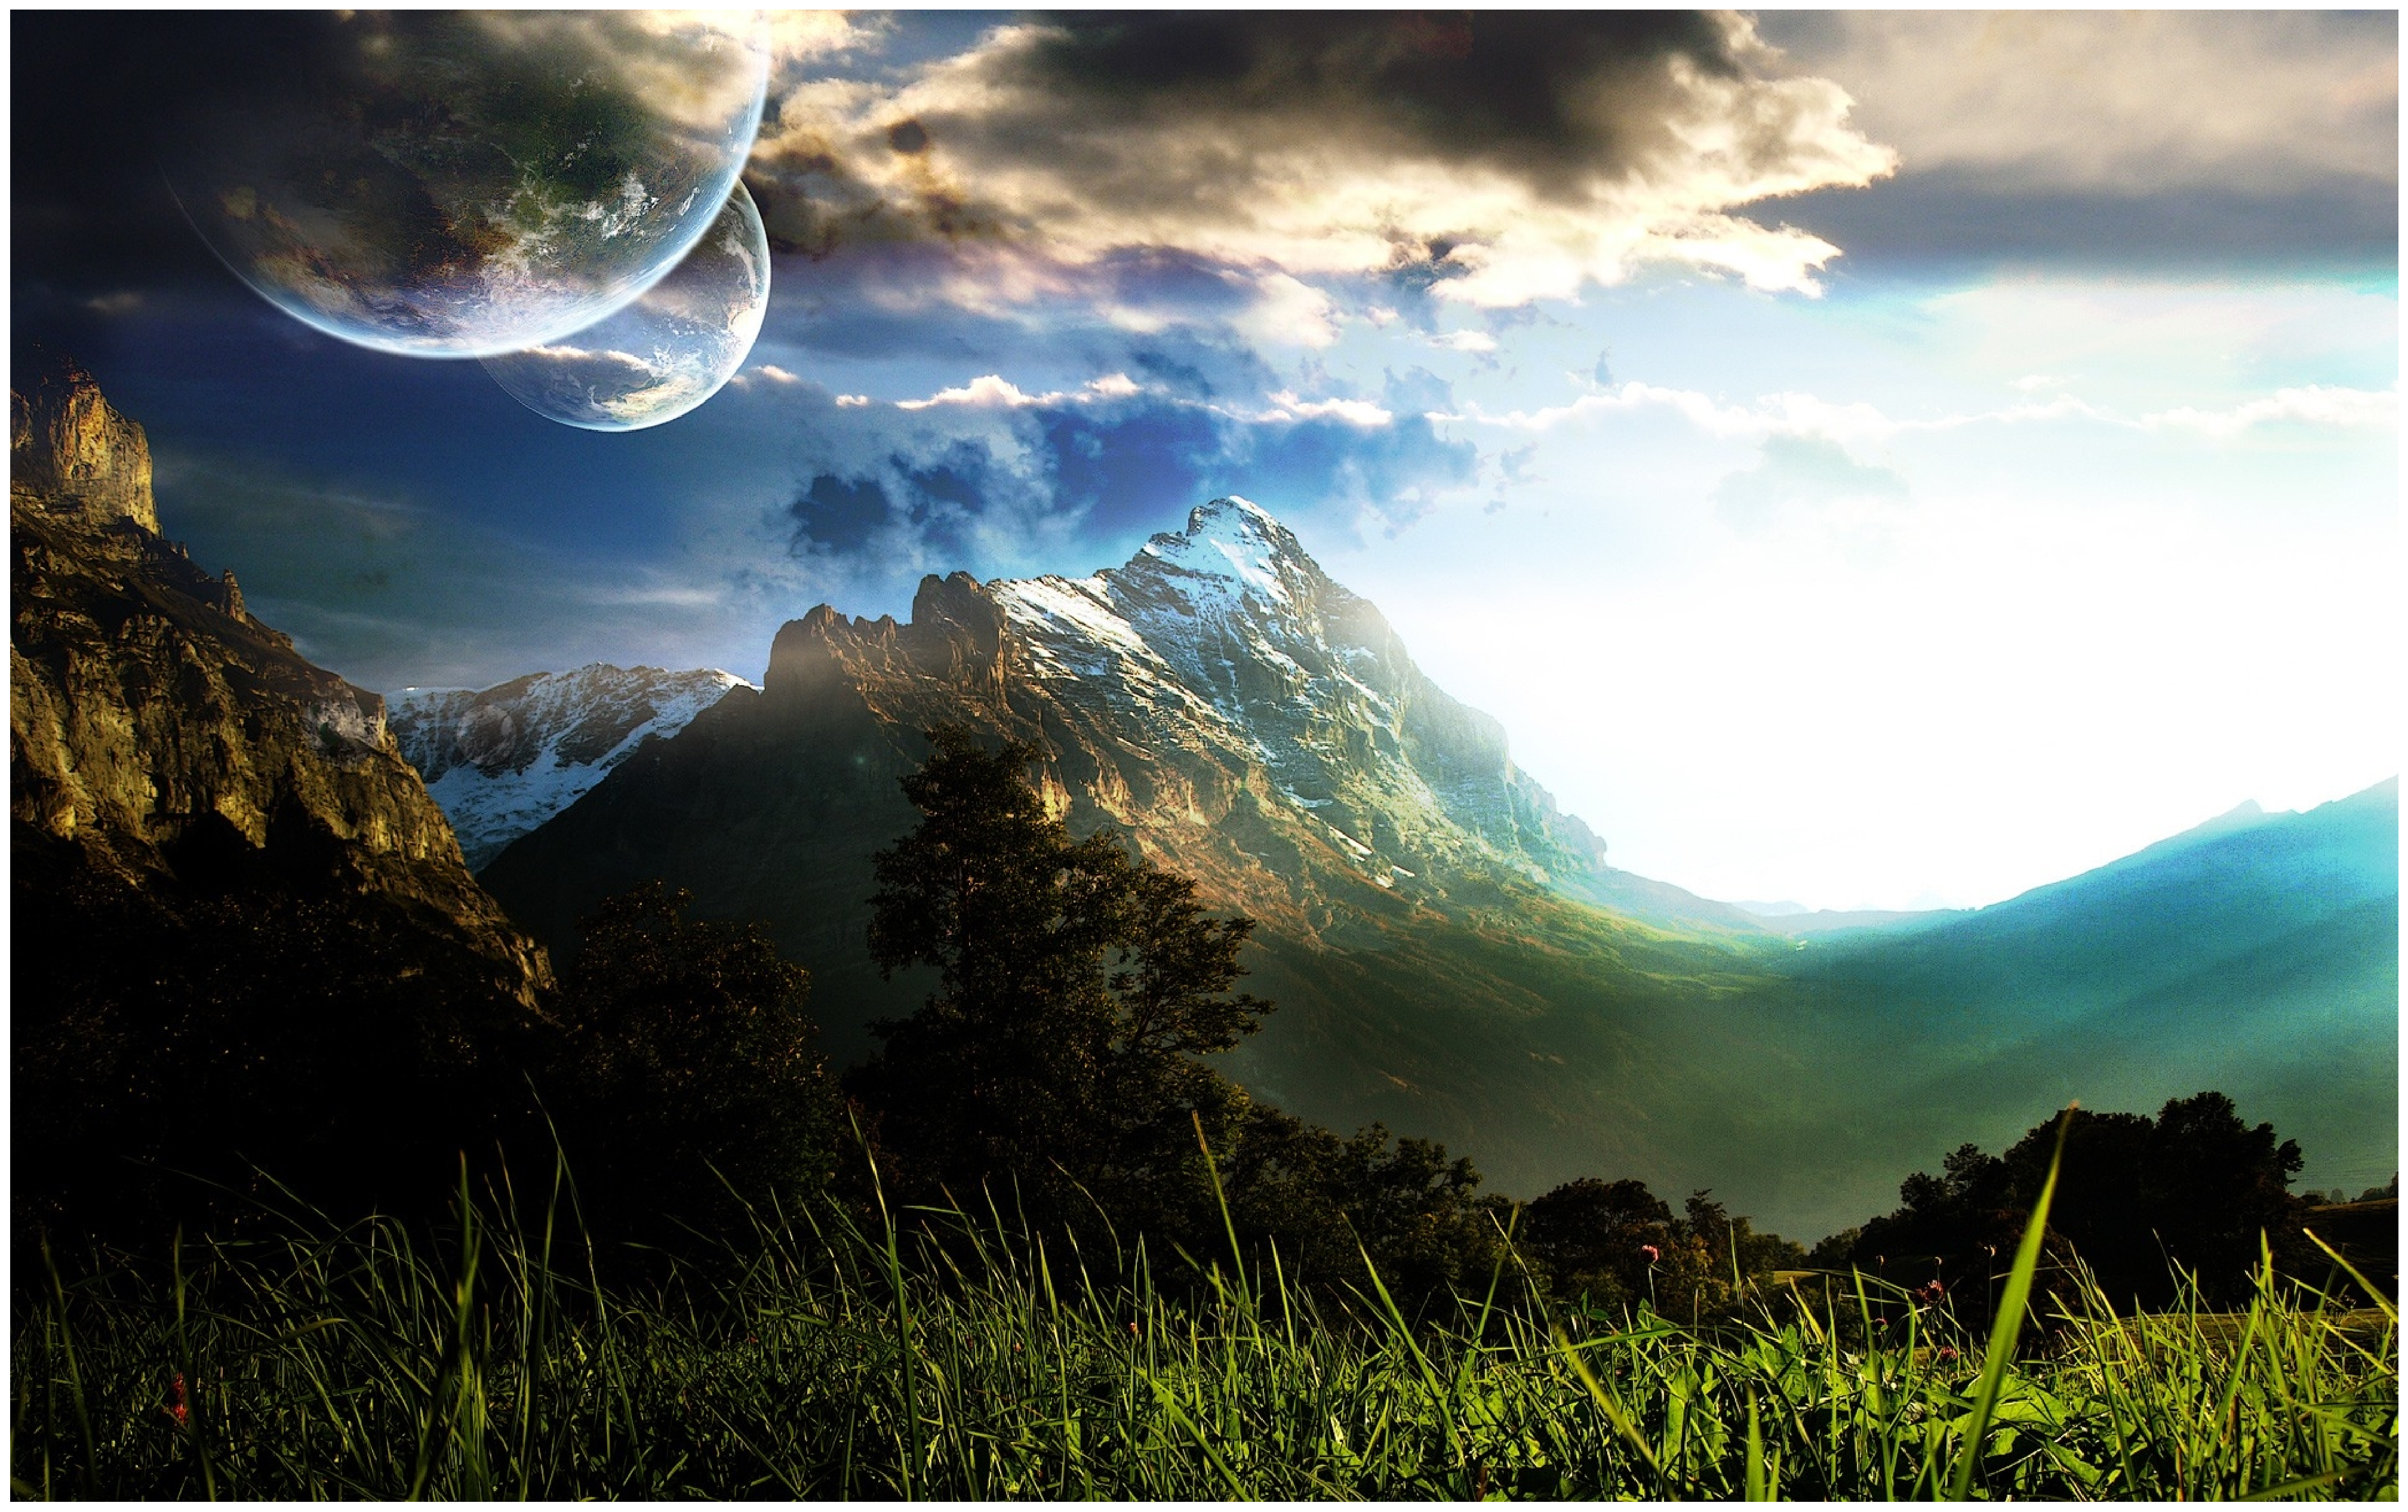
\includegraphics[scale=0.2]{figure2.eps} %中间的方括号用于设定图片大小,可以不要,大括号里是图片名字,图片大小除了用scale决定缩放比之外还可以通过width=1cm,height=2cm来指定规定大小,单位可以使用px,cm,inch等等

图片要放在同一目录下

\end{CJK}
\end{document}